\newpage
\section{Variedades diferenciales}
\label{sec.3variedades}

Las variedades diferenciales son el escenario de la geometría diferencial; todo lo que queremos estudiar en esta asignatura sucede en una. Esencialmente son espacios a los que nos podemos traer muchas propiedades y herramientas con las que sabemos trabajar en \(\mathbb{R}^n\). Espacios tan sencillos como una esfera o un toro son ejemplos de variedades, pero también lo es el espacio-tiempo de la relatividad general. En esta sección vamos a detallar qué constituye una variedad diferencial y cómo construir campos tensoriales sobre una.


\subsection{Definición}
\label{subsec.3definicion}

Vamos a dar la definición de un tirón, que así duele menos:
\paragraph{Definición} Una variedad diferencial \(\mathcal{M}\) de dimensión \(n\) es un espacio que cumple las siguientes propiedades:
\begin{myitemize}
    \item \(\mathcal{M}\) es un espacio topológico. \rnote{Espacio topológico}{Es un conjunto dotado de una familia de subconjuntos que llamamos \emph{abiertos} y que cumplen ciertas propiedades bajo uniones e intersecciones.}
    \item \(\mathcal{M}\) es Haussdorf. \rnote[2.7cm]{Haussdorf}{Para todo par de puntos distintos podemos encontrar entornos disjuntos que los separen.}
    \item \(\mathcal{M}\) es segundo contable. \rnote[4.5cm]{Segundo contable}{Podemos encontrar una base de la topología (una familia de abiertos con la que podemos construir cualquier otro abierto) numerable.}
    \item \(\mathcal{M}\) es localmente homeomorfa a \(\mathbb{R}^n\).
    \item Se puede dotar a \(\mathcal{M}\) de estructura diferencial (atlas diferenciable maximal).
\end{myitemize}
De todas estas propiedades, solo vamos a traducir las dos últimas. Las primeras son, para nosotros, detalles matemáticos que ``siempre'' se cumplen y no debemos preocuparnos. Aun así los nombramos para que quien quiera profundizar tenga hilo del que tirar.

Localmente homeomorfa a \(\mathbb{R}\) significa que existen biyecciones \(\varphi\) que van desde trozos (subconjuntos abiertos) de \(\mathcal{M}\) hasta trozos (subconjuntos abiertos) de \(\mathbb{R}^n\). Además, estas biyecciones son homeomorfismos. Visualmente, podemos imaginar que cogemos un trozo de la superficie de una esfera, \(U\in S^2\), y lo estiramos como si fuera plastilina hasta que quede plano \(\varphi(U)\in\mathbb{R}^2\).\footnote{Es como la típica imagen intuitiva de cualquier explicación de por qué un dónut y una taza son homeomorfos (topológicamente equivalentes).} A las aplicaciones \(\varphi\) se las conoce como cartas locales, cartas coordenadas o simplemente cartas, y son precisamente nuestra manera de dar coordenadas reales a los subconjuntos abiertos \(U\in\mathcal{M}\).

\begin{figure}[htbp]
    \centering
    \setlength{\unitlength}{1pt}%
\makeatletter%
\let\ASYencoding\f@encoding%
\let\ASYfamily\f@family%
\let\ASYseries\f@series%
\let\ASYshape\f@shape%
\makeatother%
\leavevmode\vbox to 99.361990pt{}%
\kern 148.545630pt%
\special{pdf:0.000000 g}%
\special{pdf:0.000000 G}%
\fontsize{12.000000}{14.400000}\selectfont%
\usefont{\ASYencoding}{\ASYfamily}{\ASYseries}{\ASYshape}%
\ASYalign(-74.272815,49.680995)(-0.500000,-0.500000){\hbox to 0pt{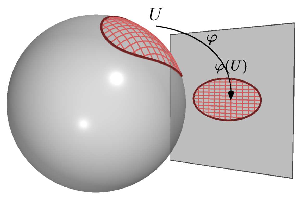
\includegraphics[hiresbb]{./figuras/carta_localmentehomeomorfo+0_0.pdf}\hss}%
\includemedia[noplaybutton,3Dlights=Headlamp,3Dmenu,3Dtoolbar=false,label=carta_localmentehomeomorfo,3Daac=27.02294933,3Dc2w=0.644217687 -0.764842187 0 -0.030569242 -0.025748117 0.999200959 -0.764231047 -0.643702931 -0.039968038 130.8902853 146.547208617 9.373133814,3Droo=205.151097333,3Dpsob=H,3Dbg=1 1 1,add3Djscript=asylabels.js]{\phantom{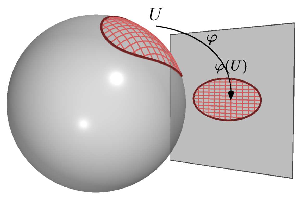
\includegraphics[hiresbb]{./figuras/carta_localmentehomeomorfo+0_0.pdf}}}{./figuras/carta_localmentehomeomorfo+0.prc}}%

    \caption{La esfera \(S^2\) es localmente homeomorfa a \(\mathbb{R}^2\). Para cada abierto \(U\in S^2\) existe un homeomorfismo \(\varphi\) que nos lleva de \(U\) a \(\varphi(U)\in\mathbb{R}^2\). El par \((U,\varphi)\) es una carta que asigna coordenadas (elementos de \(\mathbb{R}^2\)) a los puntos de \(U\in S^2\).}
    \label{fig.3-carta_localmentehomeomorfo}
\end{figure}

Que \(\mathcal{M}\) sea localmente homeomorfa a \(\mathbb{R}^n\) indica que la variedad se parece lo suficiente a \(\mathbb{R}^n\) como para poder atrevernos a extender el cálculo habitual en ella.\footnote{Técnicamente también son necesarias las propiedades de Haussdorf y de segundo contable.} La última propiedad habla justamente de eso, pero para explicarlo tenemos que aclarar primero qué es un atlas. En pocas palabras, no es más que una familia de cartas \(\varphi_i:U_i\in\mathcal{M}\rightarrow \varphi(U)\in\mathbb{R}^n\) cuyos dominios \(U_i\) cubren \(\mathcal{M}\) por completo: \(\mathcal{M} = \cup_{i}U_i\). Ahora bien, lo que queremos es un atlas \emph{diferenciable}, que significa que cuando los dominios de dos cartas cualesquiera (\(\varphi_U\) y \(\varphi_V\)) solapan (\(U\cap U'\neq \varnothing\)), el cambio de coordenadas es una función \(\mathcal{C}^\infty\) (infinitas veces diferenciable). Miremos esto del cambio de coordenadas en más detalle.

La carta \((\varphi_U, U)\) asigna a cada punto \(p\in U \subset\mathcal{M}\) unas coordenadas en \(\mathbb{R}^n\), llamémoslas \(x^i(p)\) con \(i=1,...,n\). Lo mismo vale para \((\varphi_{U'}, U')\), a cuyas coordenadas nos referiremos como \(x^{i'}(p)\). Por ser \(\varphi_U\) una biyección, existe la aplicación inversa que nos lleva de \(\mathbb{R}^n\) a \(\mathcal{M}\), \(\varphi_U^{-1}(x^1(p),...,x^n(p)) = p\). Si ahora aplicamos \(\varphi_{U'}\) sobre \(\varphi_U^{-1}(x^1(p),...,x^n(p))\), llegamos a 
\begin{equation}
    x^{i'}(p) = \varphi_{U'}\left(\varphi_U^{-1}(x^i(p))\right),
\end{equation}
es decir, la aplicación \(\varphi_{U'}\circ \varphi_U^{-1}:\mathbb{R}^n\rightarrow \mathbb{R}^n\) implementa el cambio de coordenadas. Por comodidad, en la práctica escribiremos \(x^{i'}(x^1,...,x^n)\) o simplemente \(x^{i'}(x^j)\). Ni que decir tiene que el dominio y rango de la función no son generalmente todo \(\mathbb{R}^n\).\marginexercise{Busca una forma concisa de escribir el dominio y rango de \(\varphi_{U'}\circ \varphi_U^{-1}\)} De este modo, un atlas maximal diferenciable es una colección de todas las cartas compatibles entre sí, es decir, el conjunto de todos los sistemas de coordenadas entre los cuales la transformación es \(\mathcal{C}^\infty\).

\begin{figure}[htbp]
    \centering
    \setlength{\unitlength}{1pt}%
\makeatletter%
\let\ASYencoding\f@encoding%
\let\ASYfamily\f@family%
\let\ASYseries\f@series%
\let\ASYshape\f@shape%
\makeatother%
\leavevmode\vbox to 144.530650pt{}%
\kern 177.654320pt%
\special{pdf:0.000000 g}%
\special{pdf:0.000000 G}%
\fontsize{12.000000}{14.400000}\selectfont%
\usefont{\ASYencoding}{\ASYfamily}{\ASYseries}{\ASYshape}%
\ASYalign(-88.827160,72.265325)(-0.500000,-0.500000){\hbox to 0pt{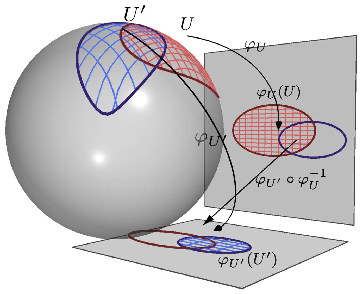
\includegraphics[hiresbb]{./figuras/cambio_coordenadas+0_0.pdf}\hss}%
\includemedia[noplaybutton,3Dlights=Headlamp,3Dmenu,3Dtoolbar=false,label=cambio_coordenadas,3Daac=32.338719409,3Dc2w=0.644217687 -0.764842187 0 -0.030569242 -0.025748117 0.999200959 -0.764231047 -0.643702931 -0.039968038 156.940551987 175.717160305 0.967523631,3Droo=245.94051638,3Dpsob=H,3Dbg=1 1 1,add3Djscript=asylabels.js]{\phantom{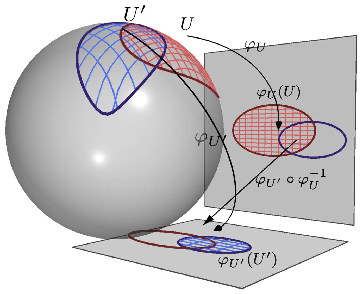
\includegraphics[hiresbb]{./figuras/cambio_coordenadas+0_0.pdf}}}{./figuras/cambio_coordenadas+0.prc}}%

    \caption{Cambio de coordenadas entre las cartas \((\varphi_U, U)\) y \((\varphi_{U'},U')\). Para llegar a \(\varphi_{U'}(U'\cap U)\) desde \(\varphi_{U}(U'\cap U)\), pasamos primero por \(U\cap U'\in\mathcal{M}\) con \(\phi^{-1}_U\) y luego aterrizamos en \(\varphi_{U'}(U'\cap U)\).}
    \label{fig.3-cambio_coordenadas}
\end{figure}

Una vez hemos ``pintado'' números reales en \(\mathcal{M}\), el siguiente paso natural es definir el espacio tangente. A ello dedicamos la siguiente subsección.

\subsection{Vectores, formas y tensores}
\label{subsec.3tensores}

Igual que en la \cref{sec.2tensores}, los tensores sobre una variedad diferencial \(\mathcal{M}\) van a ser una generalización de los vectores con más de un índice. Sin embargo, las variedades diferenciales no son necesariamente espacios vectoriales por sí mismas. Debemos antes introducir los espacios tangente y cotangente asociados.

\paragraph{Espacio tangente} Hay dos maneras de pensar en el espacio tangente de \(\mathcal{M}\) en un punto \(p\), que denotaremos por \(T_p(\mathcal{M})\). Una pasa por embeber \(\mathcal{M}\) en un espacio de dimensión mayor y considerar los hiperplanos tangentes. Esa imagen es la que refleja la \cref{fig.1-trayectorias_tangente_S2} de la \cref{sec.1motivacion}. ¿Qué podría haber malo con esa forma tan natural de construirlo? El ``problema'' con esta construcción es que es \emph{extrínseca}, en el sentido de que hay que pasar por aumentar ``artificialmente'' las dimensiones del problema y luego añadir restricciones para quedarnos con lo que nos interesa. Es muy visual, al menos para variedades de dimensión 2, pero acarrea mucho peso teórico que llevar a cuestas. 

El modo \emph{intrínseco} es más minimalista, aunque no lo parezca. Solo hace referencia a cantidades que podemos definir sobre \(\mathcal{M}\), pero requiere un poquito más de buena voluntad. Veamos cómo hacerlo. Imaginemos una función \(f:\mathcal{M}\rightarrow\mathbb{R}\) que a cada punto de \(\mathcal{M}\) le asignam un número real, como la temperatura en cada punto de la superficie de la Tierra. Componiendo \(f\) con una carta \((\varphi_U, U)\) construimos \(f\circ\varphi^{-1}_U:\varphi_U(U)\in\mathbb{R}^n \rightarrow\mathbb{R}\), que no es más que una función de varias variables de las de primero de carrera. Por aligerar la notación, no vamos a arrastrar el \(f\circ\varphi^{-1}_U\) entero, sino que reutilizaremos \(f\), que en este contexto toma como argumentos las coordenadas del punto \(x^i(p)\) en lugar del propio punto \(p\): \(f(x^i)\). En la \cref{fig.3-funcion_trayectoria} se puede ver un ejemplo de una función definida sobre la circunferencia, y su ``traducción'' a una función de variable real gracias a una carta local.

\begin{figure}[htbp]
    \centering
    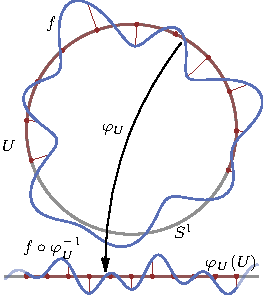
\includegraphics{figuras/funcion_trayectoria.pdf}
    \caption{Función real definida sobre la circunferencia, \(f:S^1\rightarrow\mathbb{R}\), en azul. En rojo se muestra el conjunto abierto asociado a la carta \((U, \varphi_U)\). Debajo aparece la imagen del abierto, \(\varphi_U(U)\), así como la función compuesta con las coordenadas, \(f\circ\varphi_U^{-1}\). Sobre esta última podemos aplicar la maquinaria del cálculo de forma directa.}
    \label{fig.3-funcion_trayectoria}
\end{figure}

Dado que \(f\) es una función multivariable de las conocidas, podemos aplicar las técnicas del cálculo. En concreto, podemos calcular su variación a lo largo de una trayectoria. Una trayectoria es un mapa \(\gamma:[a, b]\in\mathbb{R}\rightarrow \mathcal{M}\) que traza un camino continuo en \(\mathcal{M}\) como función de un parámetro. Ya vimos algunos ejemplos de trayectorias sobre la esfera en la \cref{fig.1-trayectorias_tangente_S2}. Lo nuevo ahora es que componiendo \(\varphi_U\) con \(\gamma\) generamos las coordenadas de la trayectoria \([\varphi_U\circ \gamma](t) = \left[\left(x^{1}\circ\gamma\right)(t),...,\left(x^n\circ\gamma\right)(t)\right]\), que son \(n\) funciones reales del parámetro \(t\). 

Como sabemos evaluar \(f\) en coordenadas (\(f\circ\varphi_U^{-1}\)), podemos obtener \(f\) a lo largo de la trayectoria \(\gamma\) como
\begin{equation}
    [f\circ \gamma](t) = [f\circ\varphi_U^{-1}\circ\varphi_U\circ \gamma](t) = f\left[\left(x^1\circ\gamma\right)(t), ..., \left(x^n\circ\gamma\right)(t)\right]
\end{equation}
que, aunque parezca intimidante, no es más que una función de una variable. La imagen mental que podemos tener es que queremos medir la temperatura en los puntos de la superficie terrestre a lo largo de una trayectoria entre Villanueva de la Cañada y Villanueva del Pardillo. Nos montamos en un coche equipados de un termómetro y hacemos el recorrido tomando medidas cuidadosamente de la temperatura y del kilometraje. Después, podemos asociarle a cada valor del kilometraje una temperatura. La coordenada es el kilometraje y la función es la temperatura. En el mundo real la temperatura no sabe nada de kilómetros. Somos nosotros quienes los introducimos, para dar sentido operacional a nuestras medidas.

Hasta aquí hemos hablado de funciones y trayectorias pero ¿dónde está el espacio tangente? Para poder describir el espacio tangente tenemos que someter a las funciones a una perrería más que ya hemos mencionado. Es el momento de derivarlas. Dada una trayectoria \(\gamma:[a, b]\in\mathbb{R}\rightarrow\mathcal{M}\) y una función \(f:\mathcal{M}\rightarrow\mathbb{R}\), definimos una \emph{derivación} de \(f\) a lo largo de \(\gamma\) en \(p=\gamma(t_p)\in\mathcal{M}\) como \marginexercise{Todo esto es un poco lioso. Dale una vuelta y haz una representación gráfica que contenga todos los elementos (variedad, trayectoria, coordenadas...).}
\begin{align}
    \nonumber
    \mathcal{D}_\gamma(f)\big|_{p} :&= \frac{\mathrm{d}}{\mathrm{d}t}[f\circ \gamma](t)\big|_{t_p} 
    = \frac{\mathrm{d}}{\mathrm{d}t} f\left[\left(x^1\circ\gamma\right)(t), ..., \left(x^n\circ\gamma\right)(t)\right]\big|_{t_p} \\
    & = 
    \frac{\partial \left(x^i\circ\gamma\right)}{\partial t}\Big|_{t_p}\frac{\partial f}{\partial x^i}\Big|_{[\varphi_U\circ\gamma](t_p)}.
\end{align}
Como tantas otras cosas, esta expresión intimida más por su apariencia que por su contenido. Lo que estamos diciendo es que \(\mathcal{D}_\gamma\) toma una función y calcula su derivada a lo largo de la trayectoria. El siguiente paso consiste en darse cuenta de que podemos aprovechar las coordenadas para reescribir esto mismo de una manera que nos insta a usar la regla de la cadena del análisis multivariable. La idea intuitiva, continuando con el ejemplo de la temperatura entre las Villanuevas, es que queremos calcular el ritmo al que las medidas cambiaban. Ese observable depende de cómo cambie la temperatura en el espacio, y de cómo de rápido nos movamos. Si la temperatura es aproximadamente constante en el espacio, da igual cuán rápidamente avance que no notaremos variación. En cambio, si la temperatura nos es homogénea, nuestra velocidad determina la magnitud de las variaciones de temperatura por unidad de tiempo.

Podemos aligerar aún más la notación suprimiendo los ``\(|_{t_p}\)'' cuando el punto en el que estemos aplicando la derivación esté claro por el contexto, y habitualmente así será. Omitiendo tales detalles, podemos escribir
\begin{align}
    \mathcal{D}_\gamma(f)_p = \frac{\partial \left(x^i\circ\gamma\right)}{\partial t}\frac{\partial }{\partial x^i} f.
\end{align}
En esta versión, prestando mucha atención a los índices, la notación sugiere que los \(\frac{\partial x^i}{\partial t}\) son componentes y los \(\frac{\partial }{\partial x^i}\) vectores de una base. Es peculiar decir que \(\frac{\partial }{\partial x^i}\) es un vector, especialmente la primera vez que uno lo encuentra así, pero los índices desde luego lo sugieren. Veamos por qué tiene sentido decir que los \(\frac{\partial }{\partial x^i}\) son vectores. 

Necesitamos comprobar que las derivaciones se pueden sumar y multiplicar por escalares. Sean dos trayectorias \(\gamma_1\), \(\gamma_2\) que se cruzan en \(p=\gamma_1(t_p) = \gamma_2(t_p)\in\mathcal{M}\). Lo que debemos asegurar es que la combinación lineal de sus derivaciones es, por sí misma, la derivación asociada a alguna trayectoria \(\gamma_3\):
\begin{align}
    \nonumber
    \mathcal{D}_{\gamma_3}(f)\big|_p &= \alpha \mathcal{D}_{\gamma_1}(f)\big|_p + \beta \mathcal{D}_{\gamma_2}(f)\big|_p \\
    &= \left[\alpha \frac{\partial \left(x^i\circ\gamma_1\right)}{\partial t}\Big|_{t_p} + \beta \frac{\partial \left(x^i\circ\gamma_2\right)}{\partial t}\Big|_{t_p} \right] \frac{\partial }{\partial x^i} f.
\end{align}
En otras palabras, tenemos que ver si existe alguna trayectoria \(\gamma_3\) cuya derivación \(\mathcal{D}_{\gamma_3}\) tenga componentes 
\begin{equation*}
    \left[\alpha \frac{\partial \left(x^i\circ\gamma_1\right)}{\partial t} + \beta \frac{\partial \left(x^i\circ\gamma_2\right)}{\partial t} \right]
\end{equation*}
en \(p\). Afortunadamente, se trata de una tarea sencilla gracias a las coordenadas que hemos implementado. Vale, por ejemplo, \(\gamma_3:[a, b]\in\mathbb{R}\rightarrow\mathcal{M}\) tal que \marginexercise{Escribe otras trayectorias posibles que den lugar a la misma derivación.} \rnote[-1.8cm]{Clase de equivalencia}{Dos elementos de un conjunto se dicen equivalentes (respecto a una relación de equivalencia) si existe una relación recíproca entre ambos. Todos los elementos relacionados entre sí forman una clase de equivalencia. Aquí el mapa entre trayectorias y derivaciones no es inyectivo, porque múltiples trayectorias van a la misma derivación. Aun así, la derivación de destino define una relación de equivalencia: todas las trayectorias que comparten derivación en \(p\) son equivalentes. El mapa entre el espacio de las clases de equivalencia y las derivaciones sí es una biyección.}
\begin{equation}
    \left(x^i\circ\gamma_3\right)(t) = x^i(p) + (t-t_p)\left[\alpha\left(x^i\circ\gamma_1\right)(t_p) + \beta\left(x^i\circ\gamma_2\right)(t_p)\right].
\end{equation}
Por supuesto, no es la única trayectoria con esas componentes en \(p\), pero es la más simple. 

\paragraph{Base del espacio tangente} A la luz del argumento previo, las derivaciones \(\frac{\partial}{\partial x^i}\), que a menudo escribiremos como \(\partial_i\) simplemente, vienen de trayectorias \(\gamma_i\) con coordenadas \((x^j\circ\gamma_i)(t_p) = x^j(p) + \delta^j_i (t-t_p)\) o equivalentes. Además, se pueden emplear para construir cualquier otra derivación como combinación lineal de las \(\partial_i\), que forman una base de \(T_p(\mathcal{M})\):
\begin{equation}
    \mathbf{v} = v^i\partial_i.
\end{equation}

Recapitulemos, que llevamos bastante camino acumulado. Olvidando un pequeño detalle, tenemos una manera precisa de asignarle a cada trayectoria una derivación. Además, las derivaciones respetan las leyes del álgebra lineal, de modo que forman un espacio vectorial. Pues bien, este espacio vectorial no es otro que el espacio tangente \(T_p(\mathcal{M})\). En primer lugar, está asociado al punto \(p\), porque es donde hemos tomado las derivadas. Además, gracias a su relación íntima con las trayectorias, posee un sentido local de direccionalidad en \(\mathcal{M}\), igual que en la perspectiva extrínseca. A \(T_p(\mathcal{M})\) le podemos preguntar la velocidad de partículas que estén en \(p\), pero nada más.

Lo último que queda por discutir respecto al espacio tangente es el cambio de base. Observemos que la base \(\mathfrak{B} = \{\partial_i\}_{i=1}^n\) está ligada a la carta \((U, \varphi_U)\), de coordenadas \(x^i\). Otra carta distinta \((U', \varphi_{U'})\) dará lugar a otra base \(\mathfrak{B}' = \{\partial_{i'}\}_{i'=1}^n\) relacionada con las coordenadas \(x^{i'}\).\footnote{Ya hicimos esta apreciación en la \cref{sec.1motivacion}, pero vuelve a ser pertinente notar que dadas unas coordenadas, podemos elegir trabajar en su base asociada o no. Tenemos libertad para complicarnos la vida lo que queramos.} ¿Cuál es la relación entre ambas bases? Bueno, como tenemos la regla de la cadena grabada a fuego, no es más que 
\begin{equation}
    \frac{\partial}{\partial x^{i'}} = \frac{\partial x^i}{\partial x^{i'}}\frac{\partial}{\partial x^{i}}.
\end{equation}
Como las derivaciones aplicadas a funciones deben ser independientes del sistema de coordenadas y de la base, tenemos que \marginexercise{Busca otra manera de demostrar la transformación de estas componentes.}
\begin{equation}
    \frac{\partial \left(x^{i'}\circ\gamma\right)}{\partial t} = 
    \frac{\partial x^{i'}}{\partial x^i}
    \frac{\partial \left(x^{i}\circ\gamma\right)}{\partial t}.
\end{equation}



\paragraph{Espacio cotangente} Una vez hemos definido el espacio tangente, incluso aún digiriendo eso de llamar \(\partial_i\) a los vectores, es más o menos directo extender las ideas de la \cref{sec.2tensores} para establecer el dual del espacio tangente, \(T^*_p(\mathcal{M})\), también llamado espacio cotangente. No es más que el conjunto de las formas lineales que actúan sobre elementos de \(T_p(\mathcal{M})\) y devuelven números reales. 

Hay asuntos relativos al espacio cotangente que debemos pararnos a comentar. Supongamos que tenemos una función \(f:\mathcal{M}\rightarrow\mathbb{R}\) y una carta \((U,\varphi_U)\). Vamos a evaluar \(f\) en puntos muy cercanos a \(p\in\mathcal{M}\) componiendo con las coordenadas:
\begin{equation}
    [f\circ\varphi^{-1}]\left(x^i(p)+v^i\right) \simeq f(p) + v^i \partial_i\left[f\circ\varphi^{-1}\right]\left(x^i(p)\right) + \mathcal{O}\left((v^i)^2\right)
\end{equation}
donde hemos aprovechado que \(\left[f\circ\varphi^{-1}\right]\) es una función multivariable para calcular su desarrollo de Taylor. El segundo término es un escalar que nos permite asociar una forma lineal a \(f\), que denotaremos por \(\mathrm{d}f\):
\begin{equation}
    \mathrm{d}f:T_p(\mathcal{M})\rightarrow \mathbb{R}\ \text{tal que}\ \mathrm{d}f\left(v^i\partial_i\right) = v^i\partial_i\left[f\circ\varphi^{-1}\right],
\end{equation}
En otras palabras, esta forma lineal se alimenta de un vector \(v^i\partial_i\) y devuelve la variación lineal de \(f\) a lo largo de la dirección del vector. En ese sentido, \(\mathrm{d}f\) codifica el ``gradiente'' de \(f\).

Antes de proseguir, hay una aclaración importante sobre la notación. El ``\(\mathrm{d}\)'' en \(\mathrm{d}f\) no significa ``diferencial'' en el sentido habitual. Por lo menos no aún. Es una notación que hemos elegido porque resulta que contiene al gradiente de \(f\) en sus tripas. En realidad, podemos aplicar \(\mathrm{d}f\) a vectores todo lo grandes que queramos, no solo a vectores infinitesimalmente pequeños, aunque nos hayamos inspirado en un desarrollo de Taylor a primer orden. Eventualmente veremos que sobre estos objetos, y generalizaciones suyas, podremos construir la teoría de la integración en variedades diferenciales, lo que justifica aún más la notación \textit{a posteriori}. 

\paragraph{Base del espacio cotangente} De todas las funciones que uno puede imaginar sobre \(\mathcal{M}\), hay unas de las que llevamos hablando desde el principio: las coordenadas de la carta \((U, \varphi_U)\). No solemos pensar en ellas como tales, pero realmente \(x^i:U\in\mathcal{M}\rightarrow\mathbb{R}\). Así, podemos componer \(\left[x^i\circ\varphi_U^{-1}\right]:\mathbb{R}^n\rightarrow\mathbb{R}\), que son las funciones simples
\begin{equation}
    \left[x^i\circ\varphi_U^{-1}\right]\left(x^1, ..., x^n\right) = x^i.
\end{equation}
A estas funciones podemos asignarles formas lineales a través de su gradiente, y dichas formas actúan sobre los vectores de la base \(\mathfrak{B}=\{\partial_i\}_{i=1}^n\) como
\begin{equation}
    \mathrm{d}x^i\left(\partial_j\right) = \partial_j(x^i\circ\varphi_U^{-1}) = \delta_j^i.
\end{equation}
Comparando con la \cref{eq.2-basedual}, queda claro que las \(\mathrm{d}x^i\) forman la base dual \(\mathfrak{B}^*\). Por tanto, cualquier forma lineal se escribe como
\begin{equation}
    \boldsymbol{\omega} = \omega_i\, \mathrm{d}x^i.
\end{equation}
Queda como ejercicio comprobar que tanto las componentes como los elementos de la base transforman adecuadamente bajo cambios de coordenadas.\marginexercise{Comprueba que la transformación de \(\omega_i\) y \(\mathrm{d}x^i\) bajo un cambio de coordenadas es el apropiado.}

Recordemos que, aunque lo hayamos omitido en la notación, todo lo que hemos construido hasta ahora, desde los vectores hasta las formas lineales, son relativos a un punto específico \(p\in\mathcal{M}\). Entra dentro de lo razonable que podamos hacer exactamente las mismas construcciones en el resto de puntos de la variedad diferencial. A la familia de todos los espacios tangentes sobre \(\mathcal{M}\) se la llama \emph{fibrado tangente}. El nombre fibrado hace referencia a que podemos imaginar los espacios tangentes un revestimiento de ``pelo'' o fibras que cubre \(\mathcal{M}\) en todos sus puntos. Se define según
\begin{equation}
    T\mathcal{M} := \bigsqcup_{p\in\mathcal{M}} T_p(\mathcal{M}) = \bigcup_{p\in\mathcal{M}} \{p\}\times T_p(\mathcal{M}).
\end{equation}
En la primera expresión, \(\bigsqcup\) enfatiza que los conjuntos que unimos son disjuntos (tienen intersección nula). Puede parecer que los espacios tangentes a una variedad deberían tener intersecciones; pensemos en una esfera. Sin embargo, ese efecto es producto de la representación que hacemos. El fibrado tangente de una esfera es un espacio 4-dimensional (2 dimensiones para especificar \(p\in\mathcal{M}\), y 2 para especificar el vector en \(T_p(\mathcal{M})\)). Eso es, precisamente, lo que hace explícito la segunda expresión. Por supuesto, también existe el fibrado cotangente, \(T^*\mathcal{M}\), que se define análogamente.

\paragraph{Campos vectoriales y 1-formas diferenciales} Una vez hemos definido el fibrado tangente (cotangente), que no son más que la familia de todos los espacios tangentes (cotangentes) a \(\mathcal{M}\) en cada punto de la variedad, podemos elegir un vector (covector) en cada uno de dichos espacios. De este modo, asignamos un vector a cada \(p\in\mathcal{M}\). A nosotros lo que nos interesa no es cualquier colección de vectores o covectores, sino aquellas colecciones que dependen suavemente de \(p\), es decir, que varían suavemente en la vecindad de todo punto de la variedad. Un campo vectorial es una colección suave de vectores, mientras que una 1-forma diferencial es una colección suave de covectores. Se especifica el ``1'' porque son el ejemplo más sencillo de las \(k\)-formas diferenciales.\rnote{Suavidad}{La manera simple de ver si una colección de vectores (covectores) es suave es comprobar que las componentes asociadas dada cualquier carta del atlas diferenciable sean funciones diferenciables (\(\mathcal{C}^\infty\)). Hay versiones más sofisticadas que prescinden de la mención a las coordenadas.} En general, encontraremos expresiones como
\begin{equation}
    \mathbf{v}\big|_p = v^i\left(x^1(p),...,x^n(p)\right) \partial_i\quad\text{o}\quad\boldsymbol{\omega}\big|_p = \omega_i\left(x^1(p),...,x^n(p)\right)\, \mathrm{d}x^i,
\end{equation}
aunque, de nuevo, a menudo eliminaremos la mención explícita al punto \(p\). Veamos algunos ejemplos.

\begin{example}
    {Campo vectorial sobre el toro
    \label{ej.3-toro_campo_vectorial}}

    Consideremos la variedad diferencial dada por la superficie del toro (dónut). Sobre esta variedad diferencial podemos definir los espacios tangentes. Por concretar, demos coordenadas \(\theta\) y \(\phi\), que representan los ángulos en las circunferencias propias del dónut. 

    \begin{figbox}
        {Campo vectorial sobre la superficie del toro. Cada vector pertenece a un plano tangente y varían suavemente cuando nos desplazamos sobre la superficie. 
        \label{fig.3-toro_campo_vectorial}}
        \setlength{\unitlength}{1pt}%
\makeatletter%
\let\ASYencoding\f@encoding%
\let\ASYfamily\f@family%
\let\ASYseries\f@series%
\let\ASYshape\f@shape%
\makeatother%
\leavevmode\vbox to 67.242090pt{}%
\kern 148.545630pt%
\special{pdf:0.000000 g}%
\special{pdf:0.000000 G}%
\fontsize{12.000000}{14.400000}\selectfont%
\usefont{\ASYencoding}{\ASYfamily}{\ASYseries}{\ASYshape}%
\ASYalign(-74.272815,33.621045)(-0.500000,-0.500000){\hbox to 0pt{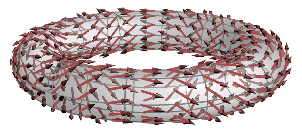
\includegraphics[hiresbb]{./figuras/toro_campo_vectorial+0_0.pdf}\hss}%
\includemedia[noplaybutton,3Dlights=Headlamp,3Dmenu,3Dtoolbar=false,label=toro_campo_vectorial,3Daac=10.099878683,3Dc2w=0.624695048 -0.780868809 0 -0.232810099 -0.186248079 0.954521404 -0.745355992 -0.596284794 -0.298142397 283.490543337 227.694497566 109.288235822,3Droo=379.655598461,3Dpsob=H,3Dbg=1 1 1,add3Djscript=asylabels.js]{\phantom{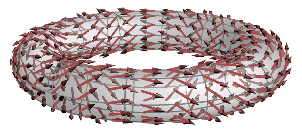
\includegraphics[hiresbb]{./figuras/toro_campo_vectorial+0_0.pdf}}}{./figuras/toro_campo_vectorial+0.prc}}%

    \end{figbox}
    
    Con \(\theta\) y \(\phi\) tenemos todo lo que necesitamos para hablar del toro, pero como vamos a dibujarlo embebido en \(\mathbb{R}^3\), emplearemos los ángulos para obtener tres coordenas cartesianas:
    \begin{align*}
        \left\{\begin{aligned}
            x &= (R + r\sin(\theta))\cos(\phi)\\
            y &= (R + r\sin(\theta))\sin(\phi)\\
            z &= r\cos(\theta)
        \end{aligned}\right.
    \end{align*}
    En cuanto al campo vectorial, por ser concretos, tomamos
    \begin{equation*}
        \mathbf{v} = v^\theta\partial_\theta + v^\phi\partial_\phi = \frac{\cos(3\phi)}{r}\partial_\theta + \frac{1}{R}\partial_\phi.
    \end{equation*}
    Para dibujarlo sobre la superficie en \(\mathbb{R}^3\) tenemos que buscar una manera de convertir las componentes \(v^\theta\) y \(v^\phi\) en \(v^{x}\), \(v^{y}\) y \(v^{z}\). Para ello recordamos la regla de la cadena, que nos permite expresar
    \begin{equation*}
        \partial_\theta = \frac{\partial x}{\partial \theta} \partial_x + \frac{\partial y}{\partial \theta} \partial_y + \frac{\partial z}{\partial \theta} \partial_z,
    \end{equation*}
    y lo mismo con \(\phi\). Así, \marginexercise{Calcula las componentes de los vectores tridimensionales correspondientes al campo vectorial del ejemplo.}
    \begin{equation*}
        v^x = \left(v^\theta \frac{\partial x}{\partial \theta} + v^\phi \frac{\partial x}{\partial \phi}\right) \partial_x,
    \end{equation*}
    y parecido con el resto de componentes.
\end{example}

Cuando introdujimos los vectores duales de \(T_p^*\mathcal{M}\) partimos del gradiente de una función \(f\), de modo que a cada función le corresponde una forma diferencial \(\mathrm{d}f\) en el punto \(p\). Extendiendo esta idea podemos utilizar \(f\) para definir una 1-forma diferencial asociada a \(f\). Dada una carta \((\varphi_U, U)\) con coordenadas \(x^j\), las componentes de \(\mathrm{d}f\) son, al menos en \(U\subset\mathcal{M}\),
\begin{equation*}
    \mathrm{d}f = \partial_i f\left(x^1,...,x^n\right) \mathrm{d}x^i,
\end{equation*}
para sorpresa de nadie. Lo que sí puede sorprender un poco es que no toda 1-forma diferencial puede obtenerse a partir del gradiente de una función \(f\). Aquellas para las que sí es posible se conocen como \emph{exactas}, mientras que al resto se las llama \emph{inexactas}. Pongamos un ejemplo.

\begin{example}
    {Forma inexacta
    \label{ej.3-formainexacta}}
    
    Consideremos la 1-forma diferencial 
    \begin{equation*}
        \boldsymbol{\omega} = \frac{y}{\sqrt{x^2+y^2}}\,\mathrm{d}x - \frac{x}{\sqrt{x^2+y^2}}\, \mathrm{d}y. 
    \end{equation*}
    Si estuviera relacionada con el gradiente de alguna función \(f\circ\varphi^{-1}\equiv f\), entonces tendríamos
    \begin{equation*}
    \partial_x f = \frac{y}{\sqrt{x^2+y^2}}\quad\text{y}\quad\partial_y f = -\frac{x}{\sqrt{x^2+y^2}}.  
    \end{equation*}
    Como las segundas derivadas conmutan, deberíamos tener \(\partial_y(\partial_x f)= \partial_x(\partial_y f)\). No obstante, en este ejemplo 
    \begin{equation*}
    \partial_y\partial_x f = \frac{y^2}{\left(x^2+y^2\right)^{3/2}}\quad\text{y}\quad\partial_x\partial_y f = -\frac{x^2}{\left(x^2+y^2\right)^{3/2}}.  
    \end{equation*}
    A las formas que sí salen del gradiente de una función se las llama \emph{exactas}, mientras que se usa \emph{inexactas} para las que no.    

    A quien no le guste la versión ``analítica'', la intuición detrás del ejemplo es la siguiente. Si tomamos las componentes y dibujamos las flechas asociadas en el plano vemos flujos circulares (mira la \cref{fig.3-forma_inexacta}). Si las flechas se correspondiesen con las componentes del gradiente de una función, podríamos integrarlas a lo largo de una trayectoria \(\gamma:[a, b]\rightarrow\mathbb{R}\). Por el teorema fundamental del cálculo, si la trayectoria fuese cerrada (\(\gamma(a)=\gamma(b) = p\)) el resultado de la integral debería dar 0. En efecto,\footnote{Hasta la \cref{subsec.3integracion} no veremos claramente cómo se define la integración de formas diferenciales sobre variedades. De momento, dejémonos llevar por la notación y nuestro conocimiento anterior sobre la integral de un gradiente.}
    \begin{equation*}
        \oint_\gamma \mathrm{d}f\, = f(p)-f(p) = 0.
    \end{equation*} 
    Sin embargo, demos una vuelta circular en sentido horario (azul). Las flechas que nos vamos encontrando siempre apuntan en la dirección de nuestro movimiento, así que todas se suman. El resultado real de la integral es, de hecho, \marginexercise{Comprobar el resultado de la integral. Para ello, cambia las coordenadas de \(x\) e \(y\) a \(r\) y \(\theta\), y reparametriza la trayectoria. Llegarás a una integral de una variable en \(\theta\) de las de toda la vida.} \rnote{Dependencia del camino}{No es solo que la integral sobre un camino cerrado no dé 0, sino que, en general, depende del camino que sigamos.}
    \begin{equation*}
        \oint_\gamma \mathrm{d}f\, = 2\pi r.
    \end{equation*} 
    donde \(r\) es el radio de la trayectoria \(\gamma\). 

    \begin{figbox}
        {Representación gráfica de una 1-forma inexacta. El resultado de integrarla depende del camino que sigamos entre el punto inicial y el final. 
        \label{fig.3-forma_inexacta}}
        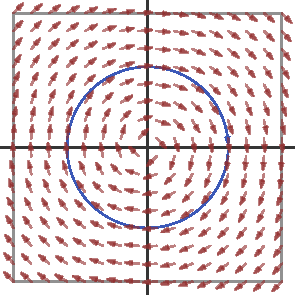
\includegraphics{figuras/ejemplo_inexacta.pdf}
    \end{figbox}

    Posiblemente, este asunto de las formas diferenciales inexactas recuerde a algunos a la termodinámica. Por ejemplo, el trabajo producido por un ciclo termodinámico es 
    \begin{equation*}
        W_\gamma = \oint_\gamma p\, \mathrm{d}V,
    \end{equation*}
    siendo \(p\) y \(V\) la presión y el volumen, respectivamente. Si \(p\, \mathrm{d}V\) fuera un diferencial exacto, un ciclo cerrado no podría producir trabajo. El calor \(Q\) tampoco tiene una forma exacta asociada. De hecho, en termodinámica se suele escribir
    \begin{equation*}
        \mathrm{\dj} W = p\,\mathrm{d}V\quad\text{y}\quad\mathrm{\dj} Q = T\,\mathrm{d}S,
    \end{equation*}
    donde \(T\) y \(S\) son la temperatura y la entropía, y la barrita en \dj denota un cambio infinitesimal, pero inexacto. La suma de ambos es la energía interna \(\mathrm{d} U = \mathrm{\dj} W + \mathrm{\dj} Q\), que sí es exacta.    
\end{example}

\paragraph{Conexión afín} Con todo el aparato conceptual que hemos introducido, estamos equipados para hacer una reflexión sobre el problema del ``transporte paralelo''. Supongamos que tenemos un vector \(\mathbf{v}_p\in T_p\mathcal{M}\) y queremos moverlo al punto \(q\in T_q\mathcal{M}\) \emph{sin alterarlo}. Si \(\mathcal{M}=\mathbb{R}^n\), podemos hacerlo sin problemas mediante la traslación afín. La idea es, simplemente, escoger el vector en el otro espacio tangente con las mismas componentes:
\begin{equation}
    T_p\mathcal{M}\ni\mathbf{v}_p = v^i\partial_i\big|_p \rightarrow \mathbf{v}_q =  v^i\partial_i\big|_q \in T_p\mathcal{M}.
\end{equation}
En otras palabras, movemos el vector y punto. Esta es una definición de transporte paralelo muy razonable en \(\mathbb{R}^n\).

Lo interesante es que, en cualquier otra variedad \(\mathcal{M}\), los distintos espacios tangentes a \(\mathcal{M}\) no tienen, a priori, ninguna relación entre ellos. Dicho de otro modo, dado un vector \(\mathbf{v}_p\in T_p\mathcal{M}\), no está claro qué vector \(\mathbf{v}_q\) le corresponde cuando nos lo llevamos a \(T_q\mathcal{M}\). Para establecer esa asociación necesitamos dotar a \(\mathcal{M}\) de una \emph{conexión afín}, que será la responsable de decirnos cómo debemos modificar las componentes de nuestro vector a medida que recorremos el camino entre \(p\) y \(q\). El ejemplo más trillado es el que se muestra en la \cref{fig.3-transporte_S2}.

\begin{figure}[htbp]
    \centering
    \setlength{\unitlength}{1pt}%
\makeatletter%
\let\ASYencoding\f@encoding%
\let\ASYfamily\f@family%
\let\ASYseries\f@series%
\let\ASYshape\f@shape%
\makeatother%
\leavevmode\vbox to 148.545630pt{}%
\kern 148.545630pt%
\special{pdf:0.000000 g}%
\special{pdf:0.000000 G}%
\fontsize{12.000000}{14.400000}\selectfont%
\usefont{\ASYencoding}{\ASYfamily}{\ASYseries}{\ASYshape}%
\ASYalign(-74.272815,74.272815)(-0.500000,-0.500000){\hbox to 0pt{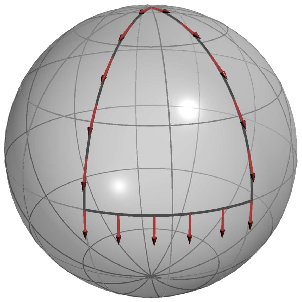
\includegraphics[hiresbb]{./figuras/transporte_paralelo_S2+0_0.pdf}\hss}%
\includemedia[noplaybutton,3Dlights=Headlamp,3Dmenu,3Dtoolbar=false,label=transporte_paralelo_S2,3Daac=22.035483465,3Dc2w=0.389418342 -0.921060994 0 -0.342073466 -0.144626342 0.928476691 -0.855183664 -0.361565854 -0.371390676 320.387033031 135.425173567 139.158813748,3Droo=374.252013679,3Dpsob=H,3Dbg=1 1 1,add3Djscript=asylabels.js]{\phantom{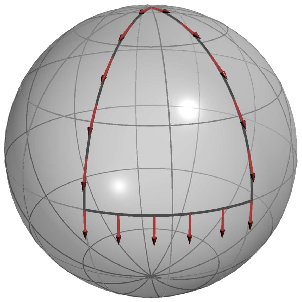
\includegraphics[hiresbb]{./figuras/transporte_paralelo_S2+0_0.pdf}}}{./figuras/transporte_paralelo_S2+0.prc}}%

    \caption{Ilustración del transporte paralelo en \(S^2\). Partiendo del polo norte, el vector rojo se transporta de la forma más paralela posible. Al volver al punto inicial ha cambiado la orientación del vector respecto al inicial.}
    \label{fig.3-transporte_S2}
\end{figure}

La conexión afín es uno de los elementos centrales en geometría diferencial. De todos modos, demoremos la exploración más detallada a la \cref{sec.4curvatura}. Nos falta extender los campos y las formas a los tensores en variedades diferenciales.

\paragraph{Tensores en variedades}

El asunto de los tensores en variedades, con todo lo que llevamos visto, es una generalización directa sin grandes complicaciones. De nuevo consideramos las aplicaciones multilineales 
\begin{equation}
    T:\underset{n}{\underbrace{T_p^*\mathcal{M}\times\cdots\times T_p^*\mathcal{M}}} \times\underset{m}{\underbrace{T_p\mathcal{M}\times\cdots\times T_p\mathcal{M}}} \rightarrow \mathbb{R},
\end{equation}
que se pueden expresar en términos de componentes con el producto tensorial:
\begin{equation}
    T = \tensor{T}{^{i_1}^{...}^{i_n}_{j_1}_{...}_{j_m}}\partial_{i_1}\otimes\cdots\otimes\partial_{i_n}\otimes\mathrm{d}x^{j_1}\otimes\cdots\otimes\mathrm{d}x^{j_m}.
\end{equation}
Si extendemos la definición de \(T\) a todos los puntos de \(\mathcal{M}\) y las componentes \(\tensor{T}{^{i_1}^{...}^{i_n}_{j_1}_{...}_{j_m}}\) son funciones suaves de las coordenadas, entonces hablamos de un campo tensorial de orden \((n,m)\). Bajo un cambio de coordenadas, la regla de la cadena aplicada \(n+m\) veces muestra que\marginexercise{Escribir explícitamente los pasos que conducen a esta regla de transformación.}
\begin{equation}
    \tensor{T}{^{i'_1}^{...}^{i'_n}_{j'_1}_{...}_{j'_m}} = 
    \frac{\partial x^{i'_1}}{\partial x^{i_1}}\cdots\frac{\partial x^{i'_n}}{\partial x^{i_n}} \frac{\partial x^{j_1}}{\partial x^{j'_1}}\cdots\frac{\partial x^{j_m}}{\partial x^{j'_m}}
    \tensor{T}{^{i'_1}^{...}^{i'_n}_{j'_1}_{...}_{j'_m}}.
\end{equation}

De todos los campos tensoriales, uno particularmente relevante es la métrica, que nos dice cómo medir vectores tangentes en cada punto de \(\mathcal{M}\):
\begin{equation}
    g = g_{ij}\, \mathrm{d}x^i\otimes \mathrm{d}x^j.
\end{equation}
Ahora que hemos metido en la mochila el asunto de las variedades, vamos a ver qué aspecto tiene la métrica en distintos casos o coordenadas.

\begin{example}
    {Métrica heredada del paraboloide hiperbólico
    \label{ej.3-metrica_paraboloide}}

    Consideremos la variedad definida por la superficie del paraboloide hiperbólico (patata \textit{pringle}). Como subconjunto de \(\mathbb{R}^3\) es
    \begin{equation*}
        \mathcal{M} = \left\{(x, y, z)\in\mathbb{R}^3 | z = x^2 - y^2\right\}
    \end{equation*}
    Puesto que sabemos medir distancias en \(\mathbb{R}^3\) con la métrica euclídea,
    \begin{equation*}
        g_{\mathbb{R}^3} = \mathrm{d}x\otimes\mathrm{d}x+\mathrm{d}y\otimes\mathrm{d}y+\mathrm{d}z\otimes\mathrm{d}z,
    \end{equation*}
    es de esperar que podamos medir distancias sobre \(\mathcal{M}\) también, heredando una métrica en su superficie \(g_\mathcal{M}\equiv g\). A continuación, mostramos el procedimiento para obtener \(g\) a partir de \(g_{\mathbb{R}^3}\). 

    En primer lugar, asignamos coordenadas (globales) a \(\mathcal{M}\). Para no complicarnos la vida, tomamos \(x^1=x\) y \(x^2=y\). Dado que coinciden con las dos primeras coordenadas cartesianas de \(\mathbb{R}^3\), sus 1-formas asociadas siguen siendo \(\mathrm{d}x\) y \(\mathrm{d}y\). Lo nuevo viene en que \(z\) ya no es una coordenada, sino una función de las coordenadas, de modo que 
    \begin{equation*}
        \mathrm{d}z = \frac{\partial z}{\partial x}\mathrm{d}x + \frac{\partial z}{\partial y}\mathrm{d}y = 2x\,\mathrm{d}x - 2y\, \mathrm{d}y.
    \end{equation*}
    Introduciendo esta relación en la propia \(g_{\mathbb{R}^3}\) llegamos a \rnote{Pullback de la métrica}{Sean dos espacios vectoriales \(W\) y \(V\) y un mapa \(f:W\rightarrow V\). Supongamos que existe un vector dual \(\boldsymbol{\nu}\in V^*\). El pullback de \(\boldsymbol{\nu}\) por \(f\) es un vector dual \(\boldsymbol{\omega}\in W^*\) cuya acción sobre vectores de \(W\) es \(\boldsymbol{\omega}(\mathbf{w}) = \boldsymbol{\nu}(f(\mathbf{v}))\). Lo que hemos hecho es el pullback de la métrica, la generalización para un tensor \((0, 2)\).} \marginexercise{Repite la misma idea para las siguientes superficies: \(z = x^2+y^2\), \(z = \cos(\sqrt{x^2+y^2})\), \(z = \sqrt{1-x^2-y^2}\) y alguna otra que te inventes.}
    \begin{equation*}
        g = 
        \left(1+4x^2\right)\mathrm{d}x\otimes\mathrm{d}x +
        \left(1+4y^2\right)\mathrm{d}y\otimes\mathrm{d}y - 
        4xy\,(\mathrm{d}x\otimes\mathrm{d}y + \mathrm{d}y\otimes\mathrm{d}x).
    \end{equation*}

    ¿Tiene sentido? Supongamos que nos movemos por la trayectoria \(x=t\), \(y = 0\). La métrica nos dice que la longitud del camino que trazamos es 
    \begin{equation*}
        \ell = \int_{t_0}^{t_1}\mathrm{d}t\,\sqrt{1+4t^2},
    \end{equation*} 
    porque tenemos que sumar los vectores infinitesimales de tamaño \(\mathrm{d}t\,\sqrt{1+4t^2}\) que nos llevan por la trayectoria. El factor \(4t^2\) corrige el hecho de que la coordenada \(z\) aumenta a medida que avanzamos en \(x\). Un mismo incremento \(\Delta x\) conlleva una mayor longitud recorrida cuanto mayor sea \(x\). Este resultado coincide, como es de esperar, con la distancia recorrida por una partícula en \(\mathbb{R}^3\) que sigue la trayectoria \(z = x^2\). En la trayectoria \(x = y = t\), lo que tenemos es 
    \begin{equation*}
        \ell = \int_{t_0}^{t_1}\mathrm{d}t\,\sqrt{1+4t^2 + 1+4t^2 -8t^2} = \int_{t_0}^{t_1}\mathrm{d}t\,\sqrt{2} = \sqrt{2}(t_1-t_0),
    \end{equation*} 
    que, de nuevo, coincide con la expectativa. En esa trayectoria \(z = 0\), luego las distancias medidas en términos de \(x\) e \(y\) son justamente las euclídeas sin factor de corrección.

    \begin{figbox}
        {Superficie del paraboloide hiperbólico. La métrica \(g\) nos permite medir la distancia de cualquier trayectoria que sigamos sobre el paraboloide, porque tiene en cuenta que, al desplazarnos en \((x(t), y(t))\), también varía la altura \(z(t)\).
        \label{fig.3-paraboloide_metrica}}
        \setlength{\unitlength}{1pt}%
\makeatletter%
\let\ASYencoding\f@encoding%
\let\ASYfamily\f@family%
\let\ASYseries\f@series%
\let\ASYshape\f@shape%
\makeatother%
\leavevmode\vbox to 144.530650pt{}%
\kern 148.545630pt%
\special{pdf:0.000000 g}%
\special{pdf:0.000000 G}%
\fontsize{12.000000}{14.400000}\selectfont%
\usefont{\ASYencoding}{\ASYfamily}{\ASYseries}{\ASYshape}%
\ASYalign(-74.272815,72.265325)(-0.500000,-0.500000){\hbox to 0pt{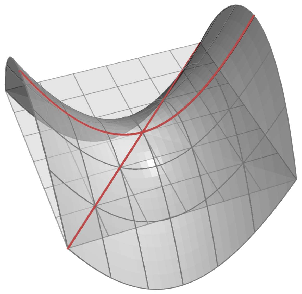
\includegraphics[hiresbb]{./figuras/paraboloide_hiperbolico+0_0.pdf}\hss}%
\includemedia[noplaybutton,3Dlights=Headlamp,3Dmenu,3Dtoolbar=false,label=paraboloide_hiperbolico,3Daac=20.925439825,3Dc2w=0.932039086 -0.362357754 0 -0.256225625 -0.659051158 0.707106781 -0.256225625 -0.659051158 -0.707106781 96.635465567 259.616728546 266.799613336,3Droo=384.517003998,3Dpsob=H,3Dbg=1 1 1,add3Djscript=asylabels.js]{\phantom{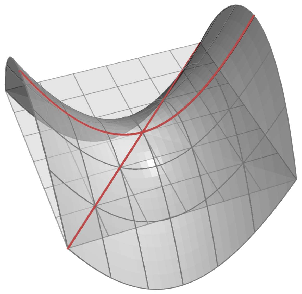
\includegraphics[hiresbb]{./figuras/paraboloide_hiperbolico+0_0.pdf}}}{./figuras/paraboloide_hiperbolico+0.prc}}%

    \end{figbox}
  
\end{example}

\begin{example}
    {Métricas lorentzianas
    \label{ej.3-metricas_lorentzianas}}
    
    En las teorías de la relatividad especial y general, el espacio-tiempo se describe como una variedad diferencial 4-dimensional a la que se dota de una (pseudo-)métrica. En relatividad especial, la métrica es la de Lorentz:\footnote{Comparando con la \cref{eq.1-intervalo_esptemp_infinitesimal}, vemos que técnicamente nos faltaba el producto tensorial entre los \(\mathrm{d}x^\mu\).} 
    \begin{equation*}
        \eta = \eta_{\mu\nu}\, \mathrm{d}x^\mu\otimes\mathrm{d}x^\nu
    \end{equation*}
    cuyas componentes son \(\eta_{\mu\nu} = \text{diag}(-1, 1, 1, 1)\) cuando usamos coordenadas cartesianas inerciales \(x^\mu = (ct, x, y, z)\).

    Decimos que \(\eta\) es una pseudométrica porque tiene un signo negativo para la coordenada temporal. Si fuera una métrica al uso, daría lugar a vectores con longitud imaginaria; en efecto,
    \begin{equation*}
        ||\partial_t|| = \sqrt{\eta_{\mu\nu}\,\mathrm{d}x^\mu(\partial_t)\mathrm{d}x^\nu(\partial_t)} =  \sqrt{\eta_{tt}} = \sqrt{-1}.
    \end{equation*}
    En lugar de distancias físicas, lo que permite medir \(\eta\) es la cantidad central de la relatividad: el intervalo espacio-temporal. Aun así, mucha de la intuición matemática y operativa que hemos ido desarrollando en variedades riemannianas,\footnote{Aquellas que tienen una métrica definida positiva que mide distancias físicas.} se trasladan directamente a las variedades lorentzianas.

    A continuación damos algunos ejemplos de métricas lorentzianas de gran relevancia:
    \begin{align*}
        \eta_\text{FLRW} =\,& -\mathrm{d}(ct)\otimes\mathrm{d}(ct) \\
        &+ R^2(t)\left(\frac{\mathrm{d}r\otimes\mathrm{d}r}{1-kr^2} + r^2 \mathrm{d}\theta\otimes\mathrm{d}\theta + r^2\sin^2\theta\, \mathrm{d}\phi\otimes\mathrm{d}\phi \right),\\
        \eta_\text{S} =&\, -\left(1-\frac{2GM}{rc^2}\right)\mathrm{d}(ct)\otimes\mathrm{d}(ct) \\
        &+\left(1-\frac{2GM}{rc^2}\right)^{-1}\mathrm{d}r\otimes\mathrm{d}r +r^2 \mathrm{d}\theta\otimes\mathrm{d}\theta + r^2\sin^2\theta\, \mathrm{d}\phi\otimes\mathrm{d}\phi.
    \end{align*}
    La primera es la métrica de Friedmann-Lema\^{i}tre-Robertson-Walker, y describe un universo homogéneo e isótropo que se expande según \(R(t)\). La constante \(k\) tiene que ver con la curvatura intrínseca del universo. Un cálculo fundamental en cosmología es averiguar la forma del factor de escala \(R(t)\) a partir de las ecuaciones de Einstein para inferir el contenido de materia y radiación. 
    
    La segunda es la métrica de Schwarzshild, que describe la solución de las ecuaciones de Einstein para un espacio-tiempo con una masa puntual \(M\) en el origen de coordenadas, con \(G\) la constante de gravitación universal de Newton. Las coordenadas escogidas son asintóticamente inerciales, es decir, ``adecuadas'' para un observador lejano. A una distancia de \(r_0 = \frac{2GM}{c^2}\) sucede algo extraño: \((\eta_\text{S})_{tt} = 0\) y \((\eta_\text{S})_{rr} = \infty\). Esa distancia es el famoso horizonte de eventos; hacia dentro tenemos un agujero negro.
    
    El horizonte de eventos da lugar a algunos efectos curiosos. Veamos qué le sucede a un rayo de luz que se aproxima radialmente hacia el origen de coordenadas. Para un rayo de luz, el intervalo espacio-temporal se anula; en más detalle, la trayectoria de un rayo de luz \(x^i(\lambda)\) tiene un vector ``velocidad'' asociado
    \begin{equation*}
        \frac{\mathrm{d}x^i}{\mathrm{d}\lambda} \partial_i.
    \end{equation*}
    El intervalo espacio-temporal asociado es 
    \begin{equation*}
        \eta_\text{S}\left( \frac{\mathrm{d}x^i}{\mathrm{d}\lambda} \partial_i, \frac{\mathrm{d}x^j}{\mathrm{d}\lambda} \partial_j\right) = -\left(1-\frac{2GM}{rc^2}\right) \left(\frac{\mathrm{d}ct}{\mathrm{d}\lambda}\right)^2 + \left(1-\frac{2GM}{rc^2}\right)^{-2} \left(\frac{\mathrm{d}r}{\mathrm{d}\lambda}\right)^2 = 0,
    \end{equation*}
    de donde
    \begin{equation*}
        \frac{\mathrm{d}ct}{\mathrm{d}\lambda}\left(1-\frac{2GM}{rc^2}\right) = \frac{\mathrm{d}r}{\mathrm{d}\lambda}.
    \end{equation*}

    Visto desde la perspectiva del observador lejano, la velocidad a la que avanza el rayo es 
    \begin{equation*}
        \frac{\mathrm{d}r}{\mathrm{d}t} = c\frac{\mathrm{d}r}{\mathrm{d}ct} = c\frac{\mathrm{d}r}{\mathrm{d}\lambda} \frac{\mathrm{d}\lambda}{\mathrm{d}ct} = c\frac{\mathrm{d}r}{\mathrm{d}\lambda} \left(\frac{\mathrm{d}ct}{\mathrm{d}\lambda}\right)^{-1}.
    \end{equation*}
    Con el resultado anterior llegamos a
    \begin{equation*}
        \frac{\mathrm{d}r}{\mathrm{d}t} = c \left(1-\frac{2GM}{rc^2}\right) = c\frac{r-r_0}{r}. 
    \end{equation*}
    Cuando el rayo está lejos del agujero negro, la velocidad medida por el observador lejano es aproximadamente \(c\). Sin embargo, para ese mismo observador, el rayo se frena al acercarse a \(r_0\), hasta detenerse por completo.
    
    Este efecto de frenado no significa que el rayo haya dejado de avanzar a la velocidad de la luz. Es un poco más sutil. La luz siempre se mueve a velocidad \(c\) si se describe su trayectoria con coordenadas localmente inerciales, es decir, en las que la métrica se reduzca a la de Minkowski. Las coordenadas que hemos usado son las más ``obvias'', pero solo son inerciales muy lejos del agujero negro. Cerca del horizonte las coordenadas son claramente no inerciales. 

    Por si no fuera algo suficientemente curioso, aún podemos darle una vuelta de tuerca importante. Es cierto que un observador lejano nunca ve el rayo alcanzar el horizonte, pero eso no es más que una ilusión producida por la elección de coordenadas. El rayo sí cae, en su trayectoria, al interior del agujero negro. El problema es que el tiempo físico que mide un reloj del observador lejano no es una buena coordenada temporal para describir el fenómeno de caída al agujero. Hay otros sistemas de coordenadas en los que sí se observa claramente que el rayo entra. En el libro de Sean Carroll se hace un análisis interesante sobre las coordenadas alternativas.\marginexercise{Leer en detalle la sección 5.6 (\textit{Schwarzshild black holes}) del libro de Carroll.}
\end{example}

\subsection{Integración de formas diferenciales en variedades}
\label{subsec.3integracion}

Lo que hemos desarrollado sobre tensores no es más que la punta del iceberg. Hay muchas maneras de profundizar en ello. Por ejemplo, podemos usarlo para extender la teoría de integración a variedades diferenciales. Quedándonos en lo superficial, vamos a ver cómo. 

\paragraph{\(k\)-formas diferenciales}Lo primero es definir una \(k\)-forma diferencial. El nombre sugiere que se trata de tensores de rango \((0, k)\), pero no nos vale cualquiera. Las \(k\)-formas son, en concreto, completamente antisimétricas. Por ejemplo, en una variedad con dimensión \(n\geq 2\), y dadas unas coordenadas \(x^k\),
\begin{align}
    \nonumber
    \omega &= \omega_{ij}\left(x^1,...,x^n\right)\, \mathrm{d}x^i\otimes\mathrm{d}x^j \\
    &= \omega_{12}\left(x^1,...,x^n\right)\,\mathrm{d}x^1 \otimes\mathrm{d}x^2 - \omega_{12}\left(x^1,...,x^n\right)\,\mathrm{d}x^2 \otimes\mathrm{d}x^1
\end{align}
es una \(2\)-forma diferencial. Efectivamente, cambiando de orden los índices en las componentes observamos que \(\omega_{ij} = -\omega_{ji}\). Otra forma de verificar la antisimetría es que\marginexercise{Comprobar que es cierto.} 
\begin{equation}
    \omega(\mathbf{u}, \mathbf{v}) = -\omega(\mathbf{v}, \mathbf{u})
\end{equation}
para dos campos vectoriales \(\mathbf{u}\) y \(\mathbf{v}\) cualesquiera. Es común denotar
\begin{equation}
    \mathrm{d}x^1 \wedge\mathrm{d}x^2 := \mathrm{d}x^1 \otimes\mathrm{d}x^2 - \mathrm{d}x^2 \otimes\mathrm{d}x^1,
\end{equation}
y se habla del producto \textit{wedge} o \emph{exterior}. Este producto puede generalizarse para combinar formas de mayor dimensión, de modo que 
\begin{align}
    \nonumber
    \mathrm{d}x^1 \wedge\mathrm{d}x^2 \wedge \mathrm{d}x^3 &= \mathrm{d}x^1 \otimes\mathrm{d}x^2\otimes \mathrm{d}x^3 + \mathrm{d}x^2 \otimes\mathrm{d}x^3\otimes \mathrm{d}x^1 + \mathrm{d}x^3 \otimes\mathrm{d}x^1\otimes \mathrm{d}x^2\\
    \nonumber
    &\phantom{=}-\mathrm{d}x^1 \otimes\mathrm{d}x^3\otimes \mathrm{d}x^2 - \mathrm{d}x^2 \otimes\mathrm{d}x^1\otimes \mathrm{d}x^3 - \mathrm{d}x^3 \otimes\mathrm{d}x^2\otimes \mathrm{d}x^1 \\
    &= \epsilon_{ijk}\, \mathrm{d}x^i \otimes\mathrm{d}x^j\otimes \mathrm{d}x^k.
\end{align}
Aquí, \(\epsilon_{ijk}\) son las componentes del símbolo de Levi-Civita,\rnote{Símbolo de Levi-Civita}{Pese a tener índices, el símbolo de Levi-Civita no es un tensor, sino una densidad tensorial. Por definición, el símbolo de Levi-Civita toma los valores que toma \emph{independientemente} del sistema de coordenadas que utilicemos. Es como un atajo de notación. La discusión en el libro de S. Carroll sobre densidades tensoriales es bastante clara.} un objeto completamente antisimétrico que vale 1 en las permutaciones pares de \((i,j,k)=(1,2,3)\), \(-1\) en las impares, y 0 en cualquier otro caso.

En general, dadas una \(k\)-forma \(\omega\) y otra \(p\)-forma \(\eta\) diferenciales, su producto \textit{wedge} es una \((k+p)\)-forma, es decir, un tensor de rango \((0, k+p)\) cuyas componentes son \marginexercise{Convéncete de que son antisimétricas.}
\begin{equation}
    (\omega\wedge\eta)_{i_1...i_{n}j_1...j_n} = \frac{1}{k!p!}\sum_{\sigma\in \mathcal{S}_{k+p}} \mathrm{sign}(\sigma)\, \omega_{i_{\sigma(1)}...i_{\sigma(k)}}
    \omega_{j_{\sigma(k+1)}...j_{\sigma(k+p)}},
\end{equation}
donde \(\mathcal{S}_r\) es el conjunto de las permutaciones de la lista \((1, 2, ..., r)\) y \(\mathrm{sign}(\sigma) = \pm 1\) dependiendo de si es una permutación par (\(+\)) o impar (\(-\)).

Vamos a ver rápidamente cómo se relacionan unas \(k\)-formas con otras. Por un lado, las \(k\)-formas diferenciales asociadas al espacio dual \(T_p^*\mathcal{M}\) forman un subespacio vectorial del espacio de los tensores de rango \((0, k)\) que se denota por \(\bigwedge^k(T_p^*\mathcal{M})\). Una base de dicho subespacio es \marginexercise{Si \(\mathcal{M}\) es una variedad diferencial de dimensión \(n\), demuestra que \(\bigwedge^k(T_p^*\mathcal{M})\) tiene dimensión \(n\choose k\).}
\begin{equation}
    \mathfrak{B}^k = \left\{\mathrm{d}x^{i_1}\wedge\cdots\wedge\mathrm{d}x^{i_k}\ |\ 1\leq i_1<\cdots<i_k\leq n\right\},
\end{equation}
de modo que una \(k\)-forma se expresa\footnote{También podríamos expandir los productos \textit{wedge} como productos tensoriales, para enfatizar que las \(k\)-formas como tensores de rango \((0, k)\).} 
\begin{equation}
    \omega = \sum_{1\leq i_1<...<i_k\leq n} \omega_{i_1...i_n} \mathrm{d}x^{i_1}\wedge\cdots\wedge\mathrm{d}x^{i_k}.
\end{equation}
La dimensión de \(\bigwedge^k(T_p^*\mathcal{M})\) es justamente \(n\choose k\), por lo que no existe \(\bigwedge^k(T_p^*\mathcal{M})\) para \(k>n\). Es más, \(\dim \bigwedge^k(T_p^*\mathcal{M}) = \dim \bigwedge^{n-k}(T_p^*\mathcal{M})\), luego existe un isomorfismo entre \(\bigwedge^k(T_p^*\mathcal{M})\) y \(\bigwedge^{n-k}(T_p^*\mathcal{M})\). No vamos a entrar en más detalle, pero un mapa interesante que nos lleva de uno a otro es la estrella de Hodge
\begin{equation}
    \star: \textstyle{\bigwedge^k}(T_p^*\mathcal{M}) \rightarrow \textstyle{\bigwedge^{n-k}}(T_p^*\mathcal{M}),
\end{equation} 
cuya acción es \marginexercise{Para coger intuición, mira los ejemplos de \href{https://en.wikipedia.org/wiki/Hodge_star_operator}{esta página de Wikipedia}.}
\begin{equation}
    \star\left(\mathrm{d}x^{i_1} \wedge \dots \wedge \mathrm{d}x^{i_k}\right) = 
    \frac{\sqrt{\left|\det g\right|}}{(n-k)!} g^{i_1 j_1} \cdots g^{i_k j_k} \varepsilon_{j_1 \dots j_n} \mathrm{d}x^{j_{k+1}} \wedge \dots \wedge \mathrm{d}x^{j_n},
\end{equation}
donde \(\det g\) es el determinante del tensor métrico.

Otra operación destacada es la derivada exterior \(\mathrm{d}\), que nos lleva de una \(k\)-forma a una \((k+1)\)-forma. Su acción es una generalización de lo que hicimos al definir los covectores a partir del gradiente de funciones:
\begin{align}
    \nonumber
    \mathrm{d}\omega &= \mathrm{d}\left(\omega_{i_1...i_k}\,\mathrm{d}x^{i_1}\wedge\cdots\wedge\mathrm{d}x^{i_n}\right)\\
    &= \sum_{j} \sum_{1\leq i_1<...<i_k\leq n} \partial_{j}\omega_{i_1...i_k}\,\mathrm{d}x^j\wedge\mathrm{d}x^{i_1}\wedge\cdots\wedge\mathrm{d}x^{i_k}.
\end{align}
La derivada exterior satisface una propiedad relevante: si se aplica dos veces sobre la misma forma el resultado es \(\mathrm{d}(\mathrm{d}\omega) = 0\), consecuencia de que \(\partial_{j}\partial_l\omega_{i_1...i_k} = \partial_{l}\partial_j\omega_{i_1...i_k}\).

\paragraph{Integración} ¿A qué ha venido todo esto? Resulta, como hemos adelantado en alguna ocasión, que las \(k\)-formas son justamente los objetos sobre los que podemos definir la integral en un sentido más abstracto:
\begin{equation}
    \int_\Sigma: \textstyle{\bigwedge^k}(T_p^*\mathcal{M}) \rightarrow \mathbb{R},
\end{equation}
donde \(\Sigma\) es una subvariedad de \(\mathcal{M}\) de dimensión \(k\). En otras palabras, la integral sobre \(\Sigma\) actúa sobre una \(k\)-forma \(\omega\) y devuelve un número real.

Centrémonos en \(k=2\) para quedarnos con la idea intuitiva. Una \(2\)-forma que nos vale es \(\mathrm{d}x^1\wedge\mathrm{d}x^2\). Vamos a hacer lo único que sabemos hacer con 2-formas, aplicarla sobre dos vectores:
\begin{align}
    \nonumber
    \left[\mathrm{d}x^1\wedge\mathrm{d}x^2\right](\mathbf{u},\mathbf{v}) &= \left[\mathrm{d}x^1\otimes\mathrm{d}x^2 - \mathrm{d}x^2\otimes\mathrm{d}x^1\right](\mathbf{u},\mathbf{v})\\
    &= u^1 v^2 - u^2v^1 = 
    \left|\begin{matrix}
        u^1 & v^1 \\ u^2 & v^2
    \end{matrix}
    \right|.
\end{align}
Quien tenga las matemáticas de secundaria frescas recordará que el determinante de una matriz \(2\times 2\) se corresponde justamente con el área (con signo) del paralelogramo formado por las columnas o filas que la componen. Una 2-forma algo más interesante sería \(\omega = f(p)\, \mathrm{d}x^1\wedge\mathrm{d}x^2\), con \(q\in\Sigma\subset\mathcal{M}\), que aplicada sobre un par de vectores devuelve el área multiplicada por \(f(x^1,...,x^n)\). Partimos, entonces, \(\Sigma\) en paralelogramos con coordenadas \((x^1)_p\) y \((x^2)_p\), y lados \(\Delta x^1\) y \(\Delta x^2\). La integral de \(\omega\) sobre \(\Sigma\) sería
\begin{equation}
    \int_\Sigma\omega \approx \sum_p \omega|_p(\Delta x^1 \partial_1, \Delta x^2 \partial_2) = \sum_p f(p) A_p,
\end{equation}
donde \(A_p\) es el área correspondiente al rectángulo \(p\)-ésimo, que no pésimo. \href{https://www.math.ucla.edu/~tao/preprints/forms.pdf}{Este texto de Terrence Tao} contiene una explicación bastante pedagógica y más detenida que la que hemos dado aquí.

La idea es, a primera vista, calcada a como concebimos la integración sobre \(\mathbb{R}^n\), aunque con un andamiaje conceptual más sofisticado para poder trasladar las normas del cálculo multi-variable a variedades diferenciales generales. En lo que sigue, vamos a hacer un par de observaciones interesantes. 

\begin{observation}
    {Formas de volumen vs. tensor métrico
    \label{obs.3-integral}}

    Hemos visto que la forma \(\mathrm{d}x^1\wedge\mathrm{d}x^2\) asigna un ``área'' a cualquier par de vectores. Por ser un tensor antisimétrico, el área tiene, adicionalmente, un signo u orientación determinado por el orden de los vectores:
    \begin{equation*}
        \left[\mathrm{d}x^1\wedge\mathrm{d}x^2\right](\mathbf{u},\mathbf{v}) = -\left[\mathrm{d}x^1\wedge\mathrm{d}x^2\right](\mathbf{v},\mathbf{u}).
    \end{equation*}
    Además, como consecuencia, la 2-forma asigna un área nula a dos vectores paralelos cualesquiera; al apuntar en la misma dirección, no definen ningún área. En general, hablamos de formas de volumen de una variedad \(n\)-dimensional como
    \begin{equation*}
        \mathrm{d}x^1\wedge\mathrm{d}x^2\wedge\cdots\wedge\mathrm{d}x^n,
    \end{equation*}
    que asigna a cada \(n\)-upla de vectores su volumen \(n\)-dimensional, con signo.\footnote{En ocasiones se dice que la 1-forma de arriba es realmente una ``densidad tensorial''. No es incorrecto, pero puede ser engañoso; hay que leer bien el contexto de la explicación. Tal y como se explica aquí, es una \(n\)-forma genuina que, en el sistema de coordenadas \(\{x^i\}\), tiene como componentes tensoriales \(\varepsilon_{i_1...i_n}\), sin perjuicio de que en otro sistema de coordenadas tenga otras componentes.}

    Sin embargo, es revelador observar que en ningún momento estamos hablando de que hayamos definido una métrica sobre la variedad en la que integramos. Habitualmente pensamos en el volumen de un paralelepípedo como algo que depende de la longitud de las aristas, y hemos dicho en varias ocasiones que la longitud de un vector está definida por la métrica. ¿Cómo puede ser que hablemos de volúmenes sin necesidad de definir una métrica? 

    La clave está en que una forma de volumen define su propia noción algebraica de volumen orientado. Esta noción no tiene por qué coincidir con el volumen físico que correspondería a la variedad a través de la métrica, pero cumple todas las propiedades esperables de un volumen orientado. En concreto, se puede demostrar que\marginexercise{Encuentra una demostración. Puedes buscar información sobre cómo introducir el símbolo de Levi-Civita y su relación con el determinante de una matriz.}
    \begin{equation*}
        \mathrm{d}x^{1'}\wedge\cdots\wedge\mathrm{d}x^{n'} = \det\left(\frac{\partial x^{i'}}{\partial x^i}\right) \mathrm{d}x^{1}\wedge\cdots\wedge\mathrm{d}x^{n},
    \end{equation*}
    donde el término en valor absoluto es el determinante de la matriz jacobiana de la transformación de coordenadas. En otras palabras,
    \begin{equation*}
        \int_\mathcal{M} \mathrm{d}x^{1'}\wedge\cdots\wedge\mathrm{d}x^{n'} = \int_\mathcal{M} \det\left(\frac{\partial x^{i'}}\partial {x^i}\right) \mathrm{d}x^{1}\wedge\cdots\wedge\mathrm{d}x^{n}.
    \end{equation*}
    Observamos que aparece justamente el determinate jacobiano de siempre cuando cambiamos de variable en una integral. 

    En el momento en que disponemos de una métrica en \(\mathcal{M}\) que nos permite medir ``físicamente'' la longitud de los vectores de \(T_p\mathcal{M}\), podemos definir una forma de volumen muy particular:
    \begin{equation*}
        \omega = \sqrt{\det g}\, \mathrm{d}x^1\wedge\cdots\wedge\mathrm{d}x^n,
    \end{equation*}
    donde \(\det g\) representa el determinante del tensor métrico expresado en las coordenadas \(x^i\). Esta forma de volumen es interesante por dos motivos. En primer lugar, resulta que \(\sqrt{\det g}\) es justamente el volumen ``físico'' asociado al paralelotopo\footnote{Generalización de paralelogramo y paralelepípedo a espacios \(n\)-dimensionales.} formado por los vectores \(\{\partial_i\}_{i=1}^n\), teniendo en cuenta el tamaño real y los ángulos entre vectores, tal y como quedan recogidos en la métrica. 
    
    El segundo motivo es que se da la peculiaridad de que en distintos sistemas de coordenadas se verifica\marginexercise{Busca una demostración en algún libro o invéntatela.}
    \begin{equation*}
        \omega = \sqrt{\det g}\, \mathrm{d}x^1\wedge\cdots\wedge\mathrm{d}x^n = \sqrt{\det g'}\, \mathrm{d}x^{1'}\wedge\cdots\wedge\mathrm{d}x^{n'},
    \end{equation*}
    siendo \(\det g'\) el determinante de la métrica expresada en las nuevas coordenadas. Es decir, sigue la misma fórmula. Lo único que cambia es que la métrica expresada en unas coordenadas u otras tiene elementos de matriz distintos y, por tanto, \(\sqrt{\det g}\neq \sqrt{\det g'}\). 

    Como ejemplo, considera \(\mathbb{R}^2\) en coordenadas cartesianas y polares. El tensor métrico en cartesianas es \(\mathrm{d}x\otimes\mathrm{d}x + \mathrm{d}y\otimes\mathrm{d}y\), cuyo determinante es 1. En cambio, en polares tenemos \(\mathrm{d}r\otimes\mathrm{d}r+r^2\mathrm{d}\theta\otimes\mathrm{d}\theta\), cuyo determinante es \(r^2\). Por tanto,
    \begin{equation*}
        \mathrm{d}x\wedge\mathrm{d}y = r\,\mathrm{d}r\wedge\mathrm{d}\theta,
    \end{equation*}
    que es el análoga a la relación entre los elementos de área ``de siempre'' \(\mathrm{d}x\, \mathrm{d}y = r\,\mathrm{d}r\,\mathrm{d}\theta\).
\end{observation}